\chapter{A new strategy for the EMEP}
\label{Sec:Numerics}



\section{Introduction}
\label{Subsec:Numerics-intro}



This chapter presents a new strategy for solving the \emep \ using the IRAM (Algorithm \ref{Alg:IRAM}, Section \ref{Subsec:evol_mats-IRAM}).
Section \ref{Subsec:Numerics-adaptive_IRAM} develops a strategy for selecting IRAM parameters based the changing behavior of the IRAM across EMEP iterates.
Section \ref{Subsec:Numerics-adaptive_IRAM_figs_and_tables} demonstrates numerically the efficiency of this new strategy.  
As compared with the original IRAM parameters used in the EMEP, we see that this new strategy decreases the number of matrix-vector products by 50-90\% for EMEPs with minimal oversamping in the phase retrieval problem (\ref{Eqn:phase_retrieval}).
Section \ref{Subsec:Numerics-correl_btwn_EMEP_and_IRAM} then examines a few EMEPs more closely to demonstrate the correlation between the clustering of the algebraically largest eigenvalues in the EMEP and the changing behavior of the IRAM for these EMEP iterates.  
We see that the new strategy from Section \ref{Subsec:Numerics-adaptive_IRAM} effectively increases the number of requested eigenvalues $j$ when the algebraically largest eigenvalues begin to cluster, thus allowing the IRAM to converge more quickly.
Note that all experiments in this chapter are available for reproduction.\footnote{\url{https://github.com/Will-Wright/low-rank-opt-rapid-eig}}










\section{The adaptive inner iteration method for the EMEP}
\label{Subsec:Numerics-adaptive_IRAM}



In this section we develop a new strategy for solving the \emep.  
This strategy uses the IRAM (Algorithm \ref{Alg:IRAM}) to handle each EMEP matrix iterate $A_k$ while adaptively changing the IRAM parameters based on the results from the EMEP iterates.
As discussed in Section \ref{Subsec:evol_mats-IRAM}, the IRAM has only two parameters: the number of requested eigenvalues $j$ and the Arnoldi decomposition (\ref{Eqn:Arnoldi_decomp}) size $m$.
As we will see, the proper choice of these parameters can greatly reduce the number of matrix-vector products required for the EMEP.





To determine how the IRAM parameters should be changed adaptively, we must understand how the computational cost (as measured by matrix-vector products) changes for various \emep \ iterates and IRAM parameters.
In the original implementation of Algorithm \ref{Alg:PGD}, all EMEP iterates were handled using the IRAM with $j=2$ requested eigenvalues and Arnoldi decomposition size $m = \min \{  \max \{ 2j, 20 \}, n \}$, where $n$ is the size of the desired signal $x$.  
This choice of $m$ is equivalent to the default parameter setting in the IRAM solver \texttt{eigs} for MATLAB and evaluates to $m=20$ for $n \geq 20$.
Yet as we saw in Section \ref{Subsec:evol_mats-spectral_props}, Figure \ref{Fig:EMEP_costs_num_mat_vecs}, the IRAM parameters $j = 2$ and $m=20$ can cause a significant increase in the number of matrix-vector products required to handle later EMEP iterates.  


To develop a new strategy for choosing the IRAM parameters $j$ and $m$ in the \emep, we will examine how the IRAM behaves for a single EMEP.  
Figure \ref{Fig:Numerics-num_matvecs_orig_vs_optimal_params} depicts the number of matrix-vector products for a range of EMEP iterates and number of requested eigenvalues $j$.

\begin{figure}[H]
\centering
\hbox{\hspace{-0.8cm} 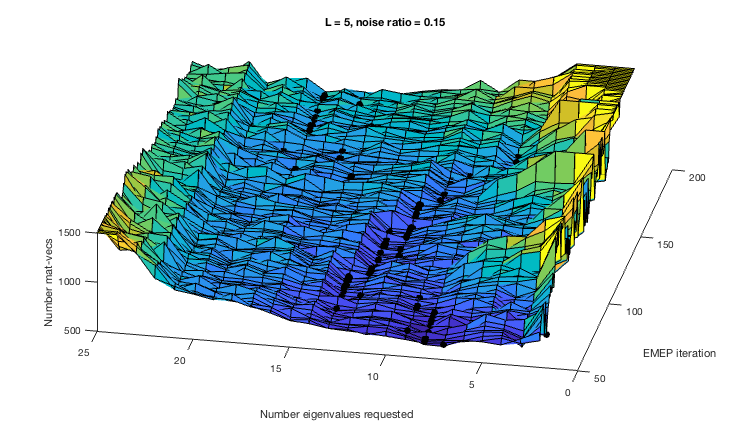
\includegraphics[scale=0.6]{Numerics-num_matvecs_orig_vs_optimal_params_1} }\vspace{1.0cm}
\hbox{\hspace{-1.6cm} 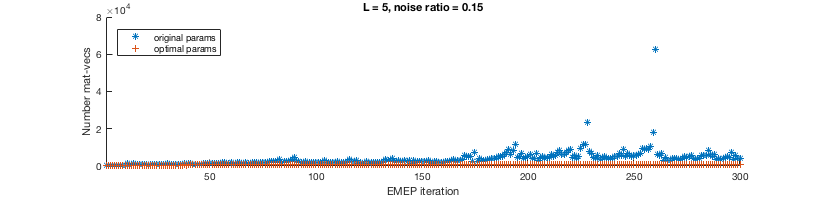
\includegraphics[scale=0.6]{Numerics-num_matvecs_orig_vs_optimal_params_2} }\vspace{0.0cm}
	\caption{
Number of matrix-vector products for an \emep \ with various IRAM parameters.
Top: Number of matrix-vector products for various EMEP iterates and number of requested eigenvalues $j$.  Arnoldi decomposition size is set to $m = 40$ and black dots indicate the \textit{optimal} parameter $j$ with the minimum number of products for each EMEP iterate.
Bottom: Plot of IRAM results for the EMEP with optimal parameters from top plot and fixed parameters $j=2$ and $m=20$.
The EMEP is from a PLGD model with Gaussian noise	 (\ref{Eqn:PhaseLift-GD_Gaussian_noise}) with noise ratio $\epsilon_\text{rel} = 0.15$, oversampling rate $L = 5$, and original signal from Figure \ref{Fig:parrot_signal_iterates} resized to $64 \times 64$ pixels.
	}
\label{Fig:Numerics-num_matvecs_orig_vs_optimal_params}
\end{figure}
% experiments.figure.noisyimage_adaptive_eig_full_exp


Figure \ref{Fig:Numerics-num_matvecs_orig_vs_optimal_params} depicts the typical behavior of the IRAM for \emeps, allowing us to develop an adaptive strategy for choosing the number of requested eigenvalues $j$.
The bottom plot in Figure \ref{Fig:Numerics-num_matvecs_orig_vs_optimal_params} demonstrates that the original EMEP parameters $j=2$ and $m=20$ cause the IRAM to slow dramatically for later EMEP iterates.
The top plot in Figure \ref{Fig:Numerics-num_matvecs_orig_vs_optimal_params} shows that the optimal choice of parameter $j$ typically changes only slightly between EMEP iterates.
However, the optimal parameter $j$ can increase quickly for later EMEP iterates (as we see around iterate 150 in the top plot in Figure \ref{Fig:Numerics-num_matvecs_orig_vs_optimal_params}).
Based on these observations, we may develop a strategy for choosing a sequence of parameters $j_1, j_2, \ldots, j_{maxit}$ using two basic heuristics.
First, we compare the two most recent choices for $j$ and the resulting number of matrix-vector products.
If these recent choices decreased the number of matrix-vector products, we continue to shift the value of $j$ in this direction; and otherwise we shift $j$ in the opposite direction.
Next, we compare the four most recent choices for $j$ and the resulting number of matrix-vector products using linear interpolation.
If these recent choices suggest the same shift as the first comparison, then we shift $j$ in this direction by two units rather than one.







We may now formally develop an adaptive strategy for choosing the number of requested eigenvalues $j_k$.
First, we select a fixed Arnoldi decomposition size $m$ and initialize $j_1=j_{min}$ and $j_2 = j_1+1$ (with default values $m=40$, $j_{min}=2$, and $j_{max} = \min\{ 30, m-5 \}$).  
At each step $k \geq 2$ we update $j_{k+1} =  j_k + \delta$, where $\delta \in \{-2, -1, 1, 2\}$ is a shift based on the number of requested eigenvalues $j_k, j_{k-1}, \ldots$ and number of matrix-vector products $t_k, t_{k-1}, \ldots$ for the previous eigenvalues problems.
The shift $\delta$ is computed as follows.
First, we determine a \textit{$2$-step shift value} $\delta_2 \in \{-1, 1\}$ based on $j_{k-1}, j_k$ and $t_{k-1}, t_k$.
If $j_k > j_{k-1}$ and $t_k < t_{k-1}$ then the number of matrix-vector products in the \emep \ decreased as the number of requested eigenvalues was increased, suggesting we should shift $j_k$ by $\delta_2 = 1$.
By the same reasoning for the other three inequality cases, we define the
\textit{$2$-step shift value} as
\begin{equation}				\label{Eqn:adaptive_delta_2}
\delta_2 = \sign(j_k - j_{k-1}) \cdot \sign(t_{k-1} - t_k),
\end{equation}
where $\sign(0)$ is defined as $1$.
Next, if $k \geq 4$ then we compute a linear interpolation of the past four requested eigenvalue numbers and matrix-vector products by solving
\begin{equation} 			\label{Eqn:adaptive_delta_4_lin_interp_prob}
\min_{\alpha, \beta} || y - \alpha e - \beta x ||,
\end{equation}
where $y$ is the vector of matrix-vector product values $t_{k-3}, t_{k-2}, t_{k-1}, t_k$, $x$ is the vector of the number of requested eigenvalues $j_{k-3}, j_{k-2}, j_{k-1}, j_k$, and $e = [1;1;1;1]$.
If the solution to (\ref{Eqn:adaptive_delta_4_lin_interp_prob}) has $\beta > 0$ then the past four eigenvalue problems suggest that $t_i$ increases with $j_i$, and thus we should decrease $j_k$.
Thus we have the \textit{$4$-step shift value}
\begin{equation}			\label{Eqn:adaptive_delta_4}
\delta_4 = -\sign(\beta),
\end{equation}
where $\beta$ is determined by (\ref{Eqn:adaptive_delta_4_lin_interp_prob}).
If $\delta_2 = \delta_4$, then the $2$-step (\ref{Eqn:adaptive_delta_2}) and $4$-step equations (\ref{Eqn:adaptive_delta_4}) both suggest we should shift in the value $\delta_2$, and we select the shift $\delta = 2\delta_2$.
If $\delta_2 \neq \delta_4$ then we rely on the $2$-step equation (\ref{Eqn:adaptive_delta_2}) and select the shift $\delta = \delta_2$.
Finally, if $j_k = j_{min}$ then we set $\delta = 1$ and if $j_k = j_{max}$ the we set $\delta = -1$.
Altogether, these steps lead to Algorithm \ref{Alg:adaptive_IRAM}.




\begin{algorithm}[H]
\caption{Adaptive inner iteration method for the \emep}	\label{Alg:adaptive_IRAM}

\begin{algorithmic}[1]
	\Statex 	\textbf{Input:} Sequence of matrices $\{ A_k \}_{k=1}^{maxit}$ from the \emep, Arnoldi decomposition (\ref{Eqn:Arnoldi_decomp})  size $m$ (default parameter $m = 40$).
	\Statex 	\textbf{Output:} \emep \ solution eigenpairs $\{ (\lambda_1^{(k)}, v_1^{(k)}) \}_{k=1}^{maxit}$ and  $\{ (\lambda_2^{(k)}, v_2^{(k)}) \}_{k=1}^{maxit}$.
	\State		\textit{Initialize:} $j_{min}=2$, $j_{max} = \min\{ 30, m-5 \}$, $j_1=j_{min}$, $t_0=-1$, $k=1$.
	\While {$k \leq maxit$}
		\State		\textit{Algorithm \ref{Alg:IRAM}:} Perform IRAM with matrix $A_k$, number of requested algebraically largest eigenvalues $j_k$, and maximum Arnoldi decomposition size $m$.  Return eigenpairs $(\lambda_1^{(k)}, v_1^{(k)} )$, $(\lambda_2^{(k)}, v_2^{(k)} )$ and number of matrix-vector products $t_k$.
		\If		{$j_k = j_{min}$}
			\State 		$j_{k+1} = j_k + 1$
		\ElsIf 	{$j_k = j_{max}$}
			\State		$j_{k+1} = j_k - 1$
		\ElsIf	{$k < 4$}
			\State		Compute $2$-step shift value $\delta_2$ from (\ref{Eqn:adaptive_delta_2}) and set $\delta = \delta_2$
			\State		$j_{k+1} = j_k + \delta$
		\Else
			\State 		Compute $2$-step shift value $\delta_2$ from (\ref{Eqn:adaptive_delta_2}) and $4$-step shift value $\delta_4$ from (\ref{Eqn:adaptive_delta_4})
			\If						{$\delta_2 = \delta_4$}
				\State		Set $\delta = 2\delta_2$
			\Else
				\State 			Set $\delta = \delta_2$
			\EndIf
			\State		$j_{k+1} =\min \{ \max \{ j_k + \delta, j_{min} \}, j_{max} \}$
		\EndIf
		\State		$k = k+1$
	\EndWhile
	\State		\textit{Return:} $\{ (\lambda_1^{(k)}, v_1^{(k)}) \}_{k=1}^{maxit}$ and  $\{ (\lambda_2^{(k)}, v_2^{(k)}) \}_{k=1}^{maxit}$.
\end{algorithmic}

\end{algorithm}



Note that the only parameter in Algorithm \ref{Alg:adaptive_IRAM} is the Arnoldi decomposition (\ref{Eqn:Arnoldi_decomp}) size $m$, which determines the size of the basis $Q_m \in \bbC^{n \times m}$ in the Arnoldi decomposition $AQ_m = Q_mH_m + r_me_m^*$.  As we will see in Section \ref{Subsec:Numerics-adaptive_IRAM_figs_and_tables}, $m$ must be sufficiently large for the shifted QR iteration (Algorithm \ref{Alg:shifted_QR_iteration}) in the IRAM to handle the \emep \ efficiently.  However,  each column of $Q_m$ is the size of the desired signal $\bar{x}$ in the phase retrieval problem (\ref{Eqn:phase_retrieval}).  Since $Q_m$ must be stored in random-access memory.  Thus the choice of $m$ is a trade-off between computational efficiency and data storage constraints.  We find that the default parameter $m=40$ strikes this balance properly.










\section{Results for the adaptive inner iteration method} 			\label{Subsec:Numerics-adaptive_IRAM_figs_and_tables}




This section demonstrates the efficiency of the adaptive inner iteration method (Algorithm \ref{Alg:adaptive_IRAM}) for solving the \emep.
We begin by demonstrating that Algorithm \ref{Alg:adaptive_IRAM} is more efficient than the original IRAM parameter settings for the \emep.
Next, we show that the Arnoldi decomposition size $m=40$ strikes a proper balance between increasing computational efficiency and minimizing data storage.
We also show that Algorithm \ref{Alg:adaptive_IRAM} is nearly optimal as a method for choosing the ideal number of requested eigenvalues $j_k$ corresponding to the minimum number of matrix-vector products necessary for each \emep \ iteration.







To examine the behavior of Algorithm \ref{Alg:adaptive_IRAM}, we consider six \emeps \ and solve each with various IRAM parameters. 
Table \ref{Tab:Numerics-num_matvecs_orig_vs_ada} depicts the total number of matrix-vector products required to solve each EMEPs with the indicated method.


\begin{table}[H]
\centering
\begin{tabular}{ |ccc|c|ccccc| }
 \hline
			  \multicolumn{3}{|c|}{n = 4,096} &  Original
			&  \multicolumn{5}{c|}{Adaptive inner iteration method (Algorithm \ref{Alg:adaptive_IRAM})}	\\
$L$ & $\epsilon_\text{rel}$ & EMEP its & $j=2, m=20$	& $m=20$  & $m=40$  & $m=60$  & $m=80$  & $m=100$   \\
 \hline
  5 &  0.05 & 300 &  406,308  &  358,195  &  198,070  &  189,401  &  192,042  &  201,270  \\ 
  5 &  0.15 & 300 & 1,099,045  &  806,412  &  258,385  &  224,048  &  214,118  &  215,392  \\ 
  5 &  0.30 &  92 &  444,697  &  175,669  &   69,510  &   56,193  &   55,146  &   54,987  \\ 
 10 &  0.05 & 153 &   80,453  &   77,768  &   68,709  &   64,300  &   68,602  &   73,754  \\ 
 10 &  0.15 & 108 &   88,317  &   65,833  &   57,231  &   53,261  &   54,388  &   55,308  \\ 
 10 &  0.30 &  54 &   72,486  &   28,799  &   25,809  &   24,699  &   25,113  &   25,491  \\ 
 \hline
\end{tabular}

\caption{
Total number of matrix-vector products for various \emeps \ with initial image from Figure \ref{Fig:parrot_signal_iterates}.  
Parameter $j$ is the number of requested eigenvalues in the IRAM (Algorithm \ref{Alg:IRAM}) and $m$ is the Arnoldi decomposition size (\ref{Eqn:Arnoldi_decomp}). 
EMEPs come from PLGD models with Gaussian noise	(\ref{Eqn:PhaseLift-GD_Gaussian_noise}) with noise ratios $\epsilon_\text{rel} = 0.05, 0.15, 0.30$, oversampling rates $L = 5$ and $10$, and an original signal from Figure \ref{Fig:parrot_signal_iterates} resized to $64 \times 64$ pixels.
} \label{Tab:Numerics-num_matvecs_orig_vs_ada}
\end{table}
% experiments.figure.noisyimage_adaptive_eig_full_exp



Table \ref{Tab:Numerics-num_matvecs_orig_vs_ada} demonstrates that Algorithm \ref{Alg:adaptive_IRAM} reduces the number of matrix-vector products from those of the original IRAM parameters for all experiments considered.
Yet this cost reduction varies significantly depending on the choice of Arnoldi decomposition (\ref{Eqn:Arnoldi_decomp}) size $m$.
Thus we seek to select a default setting for the parameter $m$ which is sufficiently large to yield the benefits of Algorithm \ref{Alg:adaptive_IRAM}.
To select the value for $m$, we examine the two experiments from Table \ref{Tab:Numerics-num_matvecs_orig_vs_ada} with $\epsilon_\text{rel} = 0.15, 0.30$ and $L=5$ which have the greatest original number of matrix-vector products, along with the greatest total decrease in cost when using Algorithm \ref{Alg:adaptive_IRAM} with a sufficiently large parameter $m$.
Figure \ref{Fig:Numerics-num_matvecs_ada_for_m_vals} singles out these two experiments, depicting the number of matrix-vector products for each \emep \ iteration.

\begin{figure}[H]
\centering
\hbox{\hspace{-1.6cm} 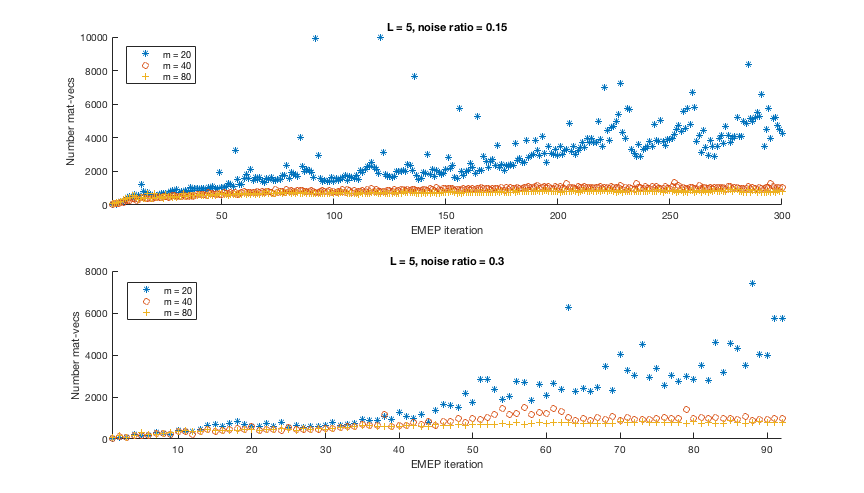
\includegraphics[scale=0.6]{Numerics-num_matvecs_ada_for_m_vals} }\vspace{0.0cm}
	\caption{Number of matrix-vector products for each \emep \ iteration from two experiments in Figure \ref{Fig:Numerics-num_matvecs_ada_for_m_vals} with various Arnoldi decomposition size $m=20, 40, 80$.}
\label{Fig:Numerics-num_matvecs_ada_for_m_vals}
\end{figure}
% experiments.figure.noisyimage_adaptive_eig_full_exp




Figure \ref{Fig:Numerics-num_matvecs_ada_for_m_vals} demonstrates that the Arnoldi decomposition size of $m=20$ is not sufficiently large to allow Algorithm \ref{Alg:adaptive_IRAM} to decrease the number of matrix-vector products.  
The dramatic matrix-vector product spikes for $m=20$ in Figure \ref{Fig:Numerics-num_matvecs_ada_for_m_vals} resemble those first seen in Figure \ref{Fig:EMEP_costs_num_mat_vecs} when solving the \emep \ with the original IRAM parameters $m=20, j=2$.
Yet when the Arnoldi decomposition size is increased to $m=40$, these cost spikes effectively disappear.
The change in number of matrix-vector products between $m=40$ and $m=80$ is minimal for each EMEP iterate.  
Thus the default parameter of $m=40$ for Algorithm \ref{Alg:adaptive_IRAM} strikes the proper balance between efficiency and data storage.






Next, we demonstrate that Algorithm \ref{Alg:adaptive_IRAM} with parameter $m=40$ is nearly optimal in the sense of choosing the number of requested eigenvalues $j_k$ which minimizes the number of matrix-vector products for each \emep \ iterate $k$.
Table \ref{Tab:Numerics-num_matvecs_opt_vs_ada} restates the number of matrix-vector products for solving the six EMEPs from Table \ref{Tab:Numerics-num_matvecs_orig_vs_ada} with an additional column depicting the minimal possible number of matrix-vector products if each value $j_k$ was chosen such that $2 \leq j_k\leq m-1$ and $j_k$ corresponds to the minimal number of matrix-vector products for the IRAM (Algorithm \ref{Alg:IRAM}) to handle matrix iterate $A_k$ with parameters $(m, j_k)$.


\begin{table}[H]
\centering
\begin{tabular}{ |ccc|c|cc|cc| }
 \hline
			&&&  Original
			&  \multicolumn{2}{c|}{Optimal $2 \leq j \leq 35$}
			&	\multicolumn{2}{c|}{Algorithm \ref{Alg:adaptive_IRAM}}	\\
$L$ & $\epsilon_\text{rel}$ & EMEP its & $j=2, m=20$	& \multicolumn{2}{c|}{$m=40$}  & \multicolumn{2}{c|}{$m=40$}   \\
 \hline
 5 &  0.05 & 300 &  406,308  &  179,807 & 56\% &  198,070 & 51\% \\ 
  5 &  0.15 & 300 & 1,099,045  &  242,003 & 78\% &  258,385 & 76\% \\ 
  5 &  0.30 &  92 &  444,697  &   58,780 & 87\% &   69,510 & 84\% \\ 
 10 &  0.05 & 153 &   80,453  &   61,948 & 23\% &   68,709 & 15\% \\ 
 10 &  0.15 & 108 &   88,317  &   51,311 & 42\% &   57,231 & 35\% \\ 
 10 &  0.30 &  54 &   72,486  &   23,217 & 68\% &   25,809 & 64\% \\ 
 \hline
\end{tabular}

\caption{Total number of matrix-vector products and percent decrease from the original IRAM parameters for various \emeps \ with initial image from Figure \ref{Fig:parrot_signal_iterates}.  Parameter $j$ is the number of requested eigenvalues in the IRAM (Algorithm \ref{Alg:IRAM}) and $m$ is the Arnoldi decomposition size (\ref{Eqn:Arnoldi_decomp}).} \label{Tab:Numerics-num_matvecs_opt_vs_ada}
\end{table}
% experiments.figure.noisyimage_adaptive_eig_full_exp

Table \ref{Tab:Numerics-num_matvecs_opt_vs_ada} demonstrates that Algorithm \ref{Alg:adaptive_IRAM} decreases the number of matrix-vector products of each \emep \ from the original IRAM parameters by a percentage comparable to that of the optimal choice for parameter $j$.
Notably, Algorithm \ref{Alg:adaptive_IRAM} is particularly effective at decreasing the number of matrix-vector products when there is a large relative difference between the number of matrix-vector products for the original IRAM parameters and the optimal parameters.
Yet in all cases, Algorithm \ref{Alg:adaptive_IRAM} is effective at choosing a parameter value $j$ within a neighborhood of the optimal value.
Figure \ref{Fig:Numerics-num_eigs_ada_vs_opt} depicts the two EMEPs from Table \ref{Tab:Numerics-num_matvecs_opt_vs_ada} with the largest and smallest relative difference between the number of matrix-vector products for the original IRAM parameters and the optimal parameters (the EMEPs with $L=5$, $\epsilon_\text{rel} = 0.15$, and $L=10$, $\epsilon_\text{rel} = 0.05$, respectively).



\begin{figure}[H]
\centering
\hbox{\hspace{-1.8cm} 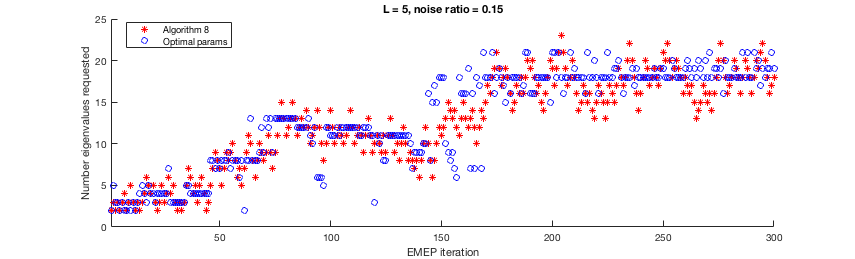
\includegraphics[scale=0.6]{Numerics-num_eigs_ada_vs_opt_1} }\vspace{0.6cm}
\hbox{\hspace{-1.8cm} 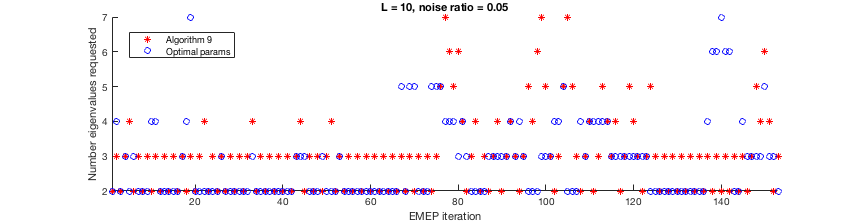
\includegraphics[scale=0.6]{Numerics-num_eigs_ada_vs_opt_2} }
\vspace{0.2cm}
	\caption{
	Number of requested eigenvalues $j$ in the IRAM (Algorithm \ref{Alg:IRAM}) for two \emeps \ from Table \ref{Tab:Numerics-num_matvecs_opt_vs_ada}.
	}
\label{Fig:Numerics-num_eigs_ada_vs_opt}
\end{figure}
% experiments.figure.noisyimage_adaptive_eig_full_exp


In both \emeps \ depicted in Figure \ref{Fig:Numerics-num_eigs_ada_vs_opt}, the number of requested eigenvalues $j$ chosen by Algorithm \ref{Alg:adaptive_IRAM} is usually within 1-3 units from the optimal parameter value.
The bottom plot in Figure \ref{Fig:Numerics-num_eigs_ada_vs_opt} suggests that Algorithm \ref{Alg:adaptive_IRAM} required relatively more matrix-vector products than the optimal value of $j$ because Algorithm \ref{Alg:adaptive_IRAM} always changes the value of $j$ by one or two units, thus shifting away from the optimal value $j=2$ for many EMEP iterates.
As we will see in Section \ref{Subsec:Numerics-correl_btwn_EMEP_and_IRAM}, this constant shifting behavior of Algorithm \ref{Alg:adaptive_IRAM} is essential due to the evolving nature of the EMEP.





\section{Correlation between EMEP spectrum and IRAM behavior}
\label{Subsec:Numerics-correl_btwn_EMEP_and_IRAM}






In this section we examine how the clustering of the algebraically largest eigenvalues in \emep \ matrix iterates affects the behavior of the IRAM (Algorithm \ref{Alg:IRAM}) for given parameters $j$ (number of requested eigenvalues) and $m$ (Arnoldi decomposition size).
As discussed in Section \ref{Subsec:evol_mats-IRAM}, the IRAM is based on the following two algorithms.
Given a Hermitian matrix $A \in \bbC^{n \times n}$, the $m$-step Arnoldi iteration (Algorithm \ref{Alg:Arnoldi_iteration}) generates a set of Ritz pairs $(\theta_1, u_1), (\theta_2, u_2), \ldots, (\theta_m, u_m)$ for $A$ with respect to $\caK_m(A, q_1)$.
Next, the $p$-step shifted QR iteration (Algorithm \ref{Alg:shifted_QR_iteration}) restarts the Arnoldi decomposition by attempting to damp the unwanted part of the spectrum using the Ritz values $\{ \theta_{j+1}, \theta_{j+2}, \ldots, \theta_m \}$ (where $m = j + p$).
In this section we present empirical evidence suggesting that the IRAM is  most efficient for an EMEP matrix iterate $A_k$ when the parameters $j$ and $m$ are sufficiently large with respect to the spectrum of $A_k$.
Specifically, $j$ must be sufficiently large so that $\lambda_{j+1}$ is not clustered with $\lambda_1, \lambda_2, \ldots, \lambda_j$, and thus the largest Ritz value $ \theta_{j+1}$ used in the $p$-step shifted QR iteration has relative separation from $\theta_j$.
And $m$ must be sufficiently large to generate an Arnoldi decomposition with accurate Ritz values to be used in the $p$-step shifted QR iteration.






To examine the correlation between the spectrum of \emep \ matrix iterates and the behavior of the IRAM, this section focuses on the two experiments from Table \ref{Tab:Numerics-num_matvecs_opt_vs_ada} with the largest relative decrease in number of matrix-vector products (i.e., the EMEPs with $L = 5$ and $\epsilon_\text{rel} = 0.15, 0.30$).
Figure \ref{Fig:Numerics-num_req_eigs_2_exps} depicts the number of requested eigenvalues $j_k$ for each EMEP iterate $k$ in these two experiments.


\begin{figure}[H]
\centering
\hbox{\hspace{-1.8cm} 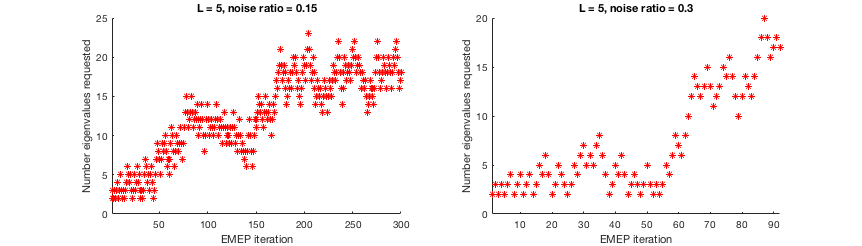
\includegraphics[scale=0.6]{Numerics-num_eigs_req_ada_2_exps} }\vspace{0.0cm}
	\caption{Number of requested eigenvalues $j$ chosen by Algorithm \ref{Alg:adaptive_IRAM} for two experiments from Table \ref{Tab:Numerics-num_matvecs_opt_vs_ada} with $\epsilon_\text{rel}=0.15, 0.30$ and $L=5$.}
\label{Fig:Numerics-num_req_eigs_2_exps}
\end{figure}
% experiments.figure.noisyimage_adaptive_eig_full_exp


For both experiments in Figure \ref{Fig:Numerics-num_req_eigs_2_exps}, the number of requested eigenvalues $j_k$ chosen by Algorithm \ref{Alg:adaptive_IRAM} changes greatly from early to later EMEP iterates.  
In particular, the experiment with $L=5$ and $\epsilon_\text{rel} = 0.30$ shows a rapid change in $j_k$ around the $60$-th iterate (where several iterates had $2$-step shift value (\ref{Eqn:adaptive_delta_2}) $\delta_2 = 1$ and $4$-step shift value (\ref{Eqn:adaptive_delta_4}) $\delta_4 = 1$,  causing Algorithm \ref{Alg:adaptive_IRAM} to increase $j_k$ by $2$).







To understand why the number of requested eigenvalues $j_k$ chosen by Algorithm \ref{Alg:adaptive_IRAM} changed greatly for the two experiments in Figure \ref{Fig:Numerics-num_req_eigs_2_exps}, we will examine the behavior of the IRAM (Algorithm \ref{Alg:IRAM}) and the structure of the \emep \ for the iterates which show greatest change in $j_k$.
Figures \ref{Fig:Numerics-surf_mvs_eig_diffs_1} depicts the number of matrix-vector products for the IRAM (top plot) and the difference between the algebraically largest eigenvalues $\lambda_{j+1} - \lambda_j$ (bottom plot) for a range of EMEP iterates $k$ and number of requested eigenvalues $j$ from the experiment with $L=5$ and $\epsilon_\text{rel} = 0.15$.
Figure \ref{Fig:Numerics-surf_mvs_eig_diffs_2} depicts the same results for the experiment with $L=5$ and $\epsilon_\text{rel} = 0.30$.
In both figures, the black dots indicate the number of requested eigenvalues $j_k$ chosen by Algorithm \ref{Alg:adaptive_IRAM} for each EMEP iterate $k$.



\begin{figure}[H]
\centering
\hbox{\hspace{-0.5cm} 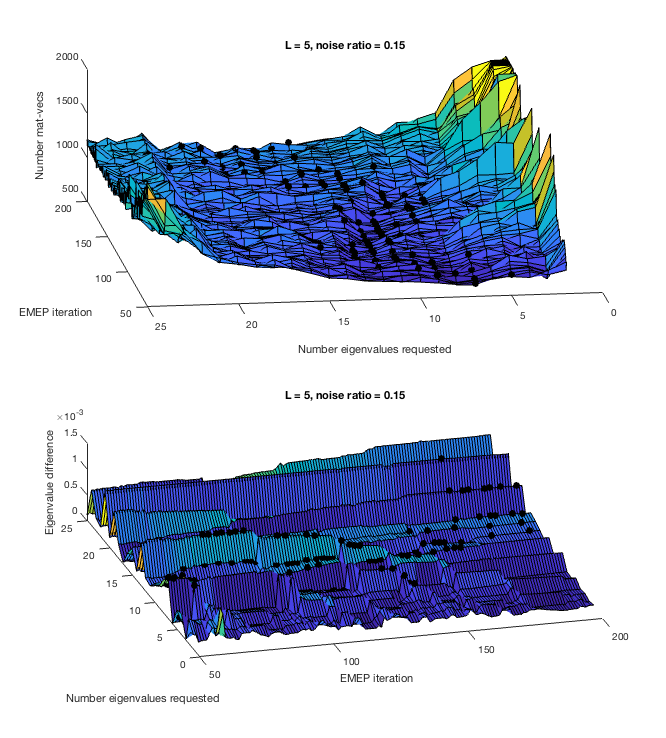
\includegraphics[scale=0.65]{Numerics-surf_num_mvs_and_eig_diffs_1} }\vspace{0.0cm}
	\caption{Behavior of Algorithm \ref{Alg:adaptive_IRAM} for the experiment from Table \ref{Tab:Numerics-num_matvecs_opt_vs_ada} with $L=5$, $\epsilon_\text{rel}=0.15$.  Top: Number of matrix-vector products (capped at 2,000 for better viewing) for each \emep \ iterate $k$ and number of requested eigenvalues $j$. Bottom: eigenvalue differences $\lambda_j - \lambda_{j+1}$ for each \emep \ iterate $k$ and number of requested eigenvalues $j$.  Black dots in both plots indicate the value $j_k$ chosen by Algorithm \ref{Alg:adaptive_IRAM}.}
\label{Fig:Numerics-surf_mvs_eig_diffs_1}
\end{figure}
% experiments.figure.noisyimage_adaptive_eig_full_exp



\begin{figure}[H]
\centering
\hbox{\hspace{-0.5cm} 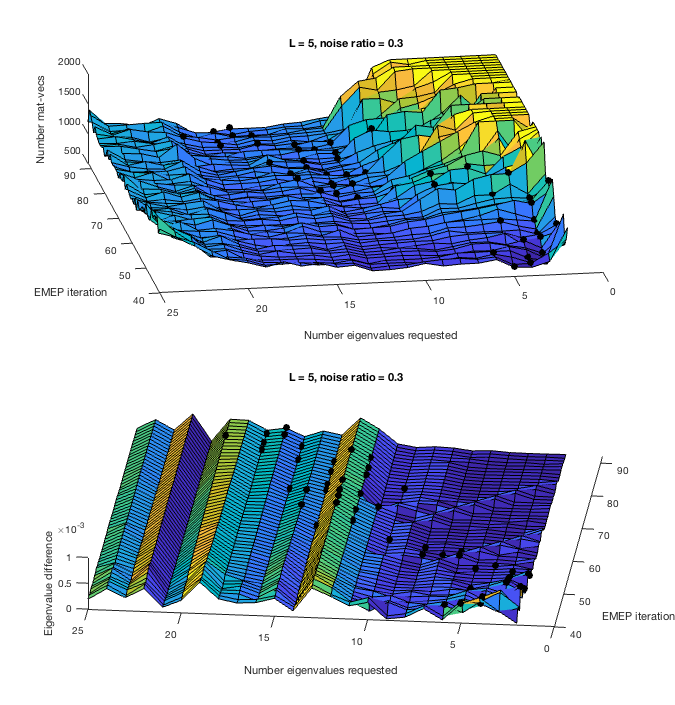
\includegraphics[scale=0.65]{Numerics-surf_num_mvs_and_eig_diffs_2} }\vspace{0.0cm}
	\caption{Behavior of Algorithm \ref{Alg:adaptive_IRAM} for the experiment from Table \ref{Tab:Numerics-num_matvecs_opt_vs_ada} with $L=5$, $\epsilon_\text{rel}=0.30$.  Top: Number of matrix-vector products (capped at 2,000 for better viewing) for each \emep \ iterate $k$ and number of requested eigenvalues $j$. Bottom: eigenvalue differences $\lambda_j - \lambda_{j+1}$ for each \emep \ iterate $k$ and number of requested eigenvalues $j$.  Black dots in both plots indicate the value $j_k$ chosen by Algorithm \ref{Alg:adaptive_IRAM}.}
\label{Fig:Numerics-surf_mvs_eig_diffs_2}
\end{figure}
% experiments.figure.noisyimage_adaptive_eig_full_exp





Figures \ref{Fig:Numerics-surf_mvs_eig_diffs_1} and \ref{Fig:Numerics-surf_mvs_eig_diffs_2} demonstrate a correlation between the number of matrix-vector products required for a given number of requested eigenvalues $j$ and the clustering of the algebraically largest eigenvalues $\lambda_1, \lambda_2, \ldots, \lambda_j, \lambda_{j+1}$.
In Figure \ref{Fig:Numerics-surf_mvs_eig_diffs_1}, the top plot shows that $j_k \approx 10$ offers the minimum number of matrix-vector products for EMEP iterates $50 \leq k  \leq 125$, while this value shifts to $15 \leq j_k \leq 20$ around EMEP iterate $k = 150$.
Correspondingly, the bottom plot in Figure \ref{Fig:Numerics-surf_mvs_eig_diffs_1} shows that the ``ridge'' of eigenvalue differences $\lambda_{j+1} - \lambda_j \approx 1 \times 10^{-3}$ for EMEP iterates $50 \leq k  \leq 125$ flattens around EMEP iterate $k = 150$, creating a region of clustered algebraically largest eigenvalues for the EMEP iterates $k \geq 150$.
Figure \ref{Fig:Numerics-surf_mvs_eig_diffs_2} depicts a similar behavior, where the number of matrix-vector products in the top plot dramatically increases for $2 \leq j  \leq 10$ around EMEP iterate $k = 60$, just as the region of eigenvalue differences flattens in the bottom plot.
For EMEP iterates $k \geq 60$, we see that $j = 12$ is the smallest parameter value necessary to minimize the number of matrix-vector products.
And likewise, for EMEP iterates $k \geq 60$ the pair $\{ \lambda_{12}, \lambda_{13} \}$ are the first pair of algebraically largest eigenvalues with greater separation than the preceding pairs.




Figures \ref{Fig:Numerics-surf_mvs_eig_diffs_1} and \ref{Fig:Numerics-surf_mvs_eig_diffs_2} suggest that for later \emep \ iterates, the number of requested eigenvalues $j$ should be large enough such that the pair $\{ \lambda_j,  \lambda_{j+1} \}$ will have sufficient separation.
Next we examine two later EMEP iterates individually to determine that the Arnoldi decomposition (\ref{Eqn:Arnoldi_decomp}) size $m$ should also be sufficiently large.
Figure \ref{Fig:Numerics-surf_mvs_for_m_vs_j} depicts the number of matrix-vector products for various $j$ and $m$ for the EMEPs from Figure \ref{Fig:Numerics-surf_mvs_eig_diffs_1} and \ref{Fig:Numerics-surf_mvs_eig_diffs_2}.


\begin{figure}[H]
\centering
\hbox{\hspace{-0.3cm} 
	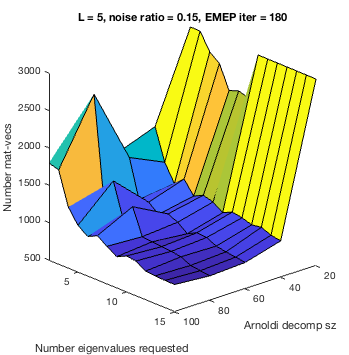
\includegraphics[scale=0.65]{Numerics-surf_mvs_for_m_vs_j_1}
	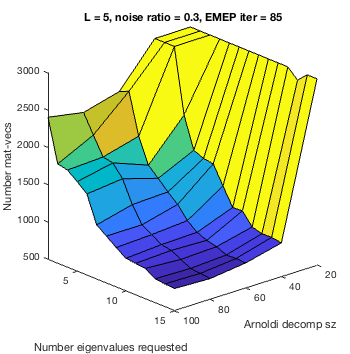
\includegraphics[scale=0.65]{Numerics-surf_mvs_for_m_vs_j_2} 
			}
	\vspace{0.0cm}
	\caption{
Number of matrix-vector products (capped at 3,000 for better viewing) for individual \emep \ iterates with varying number of requested eigenvalues $j$ and Arnoldi decomposition (\ref{Eqn:Arnoldi_decomp}) size $m$.  
Left: EMEP iterate 180 from Figure \ref{Fig:Numerics-surf_mvs_eig_diffs_1}.
Right: EMEP iterate 85 from Figure \ref{Fig:Numerics-surf_mvs_eig_diffs_2}.
	}
\label{Fig:Numerics-surf_mvs_for_m_vs_j}
\end{figure}
% experiments.figure.noisyimage_adaptive_eig_full_exp


Figure \ref{Fig:Numerics-surf_mvs_for_m_vs_j} suggests that we should not select IRAM parameters below $j = 9$ and $m = 40$ for the EMEP iterate in the left plot, or $j = 12$ and $m = 40$ for the EMEP iterate in the right plot.  
Yet there is no significant benefit to selecting larger parameter values.
These minimum parameter values for $j$ again correspond to the desired eigenvalue differences from Figures \ref{Fig:Numerics-surf_mvs_eig_diffs_1} and \ref{Fig:Numerics-surf_mvs_eig_diffs_2}, respectively.
The IRAM behavior depicted in Figures \ref{Fig:Numerics-surf_mvs_eig_diffs_1}, \ref{Fig:Numerics-surf_mvs_eig_diffs_2}, and \ref{Fig:Numerics-surf_mvs_for_m_vs_j} suggests that we should select a value $j$ such that the pair $\{ \lambda_j,  \lambda_{j+1} \}$ will have sufficient separation.
This choice of $j$ may be a necessary component in allowing the $p$-step shifted QR iteration (Algorithm \ref{Alg:shifted_QR_iteration}) in the IRAM to shift away the unwanted part of the spectrum.
Additionally, the value $m=40$ appears to be the minimum Arnoldi decomposition size sufficient for identifying accurate Ritz values $\{ \theta_{1}, \theta_{2}, \ldots, \theta_m \}$, of which the values $\{ \theta_{j+1}, \theta_{j+2}, \ldots, \theta_m \}$ are to be used in the $p$-step shifted QR iteration.







As we have seen in this chapter, Algorithm \ref{Alg:adaptive_IRAM} is an efficient strategy for using the IRAM (Algorithm \ref{Alg:IRAM}) to handle the \emep.  
The behavior of Algorithm \ref{Alg:adaptive_IRAM} corresponds to the evolving spectrum of the EMEP and appears to be promoting convergence of the IRAM by properly utilizing the two primary subroutines in the IRAM.
We now proceed to demonstrate the efficiency of Algorithm \ref{Alg:adaptive_IRAM} for a wider variety of \emeps \ and summarize the contributions in this dissertation.






